\documentclass[a4paper,10pt]{article}
\usepackage[utf8]{inputenc}
\usepackage[spanish]{babel}
\usepackage[affil-it]{authblk}
\usepackage{enumerate}
\usepackage{graphicx}
\usepackage{hyperref}
\usepackage{amsmath}
\usepackage{amssymb}
\usepackage{cancel}
\usepackage[usenames, dvipsnames]{color}
\usepackage{tikz}
\usepackage{multimedia}
\usepackage{subcaption} %Multiple images
\usepackage{multicol} % Multiple columns
\usepackage{float}
\usepackage{cleveref}
 \usepackage{relsize} %bigger math symbols
\usepackage[margin=1.4in]{geometry}
\usepackage[labelfont=bf]{caption}
\usepackage[titletoc,toc,title]{appendix}
\usepackage{enumitem}
\usetikzlibrary{calc}
\numberwithin{equation}{section}

%Appendices in spanish
\renewcommand{\appendixname}{Ap\'endices}
\renewcommand{\appendixtocname}{Ap\'endices}
\renewcommand{\appendixpagename}{Ap\'endices}

%Zero delimiter
\newcommand{\zerodel}{.\kern-\nulldelimiterspace}

%Columns separation
\setlength{\columnsep}{1cm}

%Indentation
\setlength{\parindent}{0ex}

%Multiple References

\crefrangelabelformat{equation}{(#3#1#4--#5\crefstripprefix{#1}{#2}#6)}

\usepackage{xparse}
\ExplSyntaxOn
\NewDocumentCommand{\mref}{m}{\quinn_mref:n {#1}}
\seq_new:N \l_quinn_mref_seq
\cs_new:Npn \quinn_mref:n #1
 {
  \seq_set_split:Nnn \l_quinn_mref_seq { , } { #1 }
  \seq_pop_right:NN \l_quinn_mref_seq \l_tmpa_tl
  ( % print the left parenthesis
  \seq_map_inline:Nn \l_quinn_mref_seq
    { \ref{##1},\nobreakspace } % print the first references
  \exp_args:NV \ref \l_tmpa_tl 
  ) 
 }
\ExplSyntaxOff


%Boxes

\newcommand*{\boxcolor}{blue}
\makeatletter
\renewcommand{\boxed}[1]{\textcolor{\boxcolor}{%
\tikz[baseline={([yshift=-1ex]current bounding box.center)}] \node [rectangle, minimum width=1ex,rounded corners,draw] {\normalcolor\m@th$\displaystyle#1$};}}
 \makeatother

%Constantes
\newcommand{\euler}{\mathrm{e}}
\newcommand{\im}{i}

%Lemas, teoremas, definiciones y pruebas
\newcommand{\definicion}{\textbf{Definición: }}
\newcommand{\lema}{\textbf{Lema: }}
\newcommand{\teorema}{\textbf{Teorema: }}
\newcommand{\prueba}{\textbf{Prueba: }}
\newcommand{\proposicion}{\textbf{Proposición: }}
\newcommand{\corolario}{\textbf{Corolario: }}


%opening
\title{Mecánica Clásica Tarea \# 8}
\author{Favio Vázquez\thanks{Correo: favio.vazquezp@gmail.com}}\affil{Instituto de Ciencias Nucleares. Universidad Nacional Autónoma de México.}
\date{}

\begin{document}

\makeatletter
\def\@maketitle{%
  \newpage
  \null
  \vskip 2em%
  \begin{center}%
  \let \footnote \thanks
    {\Large\bfseries \@title \par}%
    \vskip 1.5em%
    {\normalsize
      \lineskip .5em%
      \begin{tabular}[t]{c}%
        \@author
      \end{tabular}\par}%
    \vskip 1em%
    {\normalsize \@date}%
  \end{center}%
  \par
  \vskip 1.5em}
\makeatother

\maketitle

\section{Problema 1}

Construya un atlas para el toro de dos dimensiones.

\vspace{.3cm}

\underline{Solución:} \vspace{.3cm}

\section{Problema 2}

Demuestre que la estructura de espacio vectorial que se dio al conjunto de clases de 
tangencia de curvas que pasan por un punto de una variedad diferencial, es independiente 
de las cartas utilizadas y de las curvas representativas escogidas en cada clase.

\vspace{.3cm}

\underline{Solución:} \vspace{.3cm}

Durante toda la prueba utilizaremos el convenio de suma de Einstein, el cual nos dice 
que un índice que aparece dos veces en un término matemático, una vez como un 
superíndice y una vez como un subíndice, es sumado sobre el rango entero de ese 
índice. 

\vspace{.3cm}

Queremos pensar en un campo vectorial sobre una variedad diferencial $M$ como un 
mapeo $\xi$ que asigna a cada punto $p \in M$ un vector tangente $\xi_p \in T_p M$, 
junto con alguna suposición de continuidad o diferenciabilidad. Pero como bien 
se establece en las notas del curso, antes de que podamos pensar en ese objeto 
como un mapeo, debemos definir el conjunto que será su rango. Esto nos lleva a la 
definición de ``haz tangente''.

\vspace{.3cm}

\definicion Sea una variedad diferencial $M$, definimos el \emph{haz tangente} de 
$M$, denotado por $TM$, como la unión disjunta de espacios tangentes en todos 
los puntos de $M$:

\begin{equation}
 TM = \underset{p \in M}{\coprod} T_p M.
\end{equation}

Escribiremos un elemento de esta unión disjunta como el par ordenado $(p,\xi)$, 
con $p \in M$ y $\xi \in T_pM$. El haz tangente viene equipado con un un mapeo 
de proyección natural $\pi = TM \rightarrow M$, que mapea cada vector en $T_p M$ 
al punto $p$ en el cual es tangente: $\pi(p,\xi) = p$. El siguiente lema 
muestra que $TM$ puede pensarse como una variedad diferenciable en si mismo.

\vspace{.3cm}

\lema Para cualquier variedad diferencial $M$ de $n$ dimensiones, el haz tangente 
$TM$ tiene una topología natural y una estructura diferenciable que lo hace 
una variedad diferencial de $2n$ dimensiones. Con esta estructura, $\pi: TM \rightarrow M$ 
es un mapeo diferenciable.

\vspace{.3cm}

\prueba Comenzamos por definir los mapeos que se convertirán en nuestras cartas 
diferenciables. Dada una carta diferenciable $(U,\phi)$, sean $(q^1,\dots,x^n)$ 
las funciones coordenadas de $\phi$, y definimos un mapeo $\phi': \pi^{-1}(t) \rightarrow \mathbb{R}^{2n}$ 
por 

\begin{equation}
 \phi' \left( v^i \left\zerodel\frac{\partial}{\partial q^i}\right|_p \right) = 
 (q^1(p),\dots,q^n(p),v^1,\dots,v^n).
\end{equation}

Su conjunto imagen es $\phi(U) \times \mathbb{R}^n$, que es un subconjunto abierto 
de $\mathbb{R}^{2n}$. Es una biyección sobre su imagen, debido a que su inversa 
puede escribirse explícitamente como

\begin{equation}
 \phi'^{-1}(q^1(p),\dots,q^n(p),v^1,\dots,v^n) = v^i \left\zerodel\frac{\partial}{\partial q^i}\right|_{\phi^{-1}(q)}.
\end{equation}

Sean ahora dos cartas diferenciales dadas $(U,\phi)$ y $(V,\psi)$ para $M$, y 
sean $(\pi^{-1}(U),\phi')$, $(\pi^{-1}(V),\psi')$ las cartas correspondientes sobre 
$TM$. Los conjuntos $\phi'(\pi^{-1}(U)\cap\pi^{-1}(V)) = \phi(U \cap V) \times \mathbb{R}^n$ 
y $\psi'(\pi^{-1}(U)\cap\pi^{-1}(V) = \psi(U \cap V) \times R^n$ son ambos abiertos 
en $\mathbb{R}^{2n}$, y el mapeo de transición 
$\psi' \circ \phi'^{-1}: \phi(U \cap V) \times \mathbb{R}^n \rightarrow 
\psi(U\cap V)\times \mathbb{R}^n$ puede escribirse explícitamente como\footnote{Ver problema 4.}

\begin{align}
\begin{split}
 \psi' \circ \phi'^{-1}(q^1(p),\dots,q^n(p),v^1,\dots,v^n) = \\
 \left(q'^1(q),\dots,q'^n(q),\frac{\partial q'^1}{\partial q^j}(q)v^j, 
 \dots,\frac{\partial q'^n}{\partial q^j}(q)v^j\right).
 \end{split}
\end{align}

El cual es claramente diferenciable. Si escogemos una cobertura contable 
$\{U_i\}$ sobre $M$ un dominio de coordenadas diferenciables, obtenemos 
una cobertura contable sobre $TM$ con un dominio de coordenadas ${\pi^{-1}(U_i)}$,
con lo cual cumple con las condiciones para la construcción de una variedad 
diferencial. También puede probarse que satisface la condición de Hausdorff 
lo cual no haremos aquí. Por último para ver que $\pi$ es diferenciable, 
notamos que su representación en coordenadas con respecto a las cartas 
$(U,\phi)$ para $M$ y $(\pi^{-1}(U),\phi')$ para $TM$ es $\pi(q,v))q$.

$\hspace{12cm} \square$

Podemos ahora definir lo que queríamos, un campo vectorial.

\vspace{.3cm}

\definicion Si $M$ es una variedad diferencial, un campo vectorial 
sobre $M$ es una sección del mapeo $\pi:TM \rightarrow M$. De forma 
más concreta, un campo vectorial es un mapeo continuo $\zeta:M \rightarrow TM$, 
usualmente escrito $p \mapsto \zeta_p$, con la propiedad que 

\begin{equation}
 \pi \circ \zeta = \text{Id}_M,
\end{equation}

o de forma equivalente, $\zeta_p \in T_p M \forall p \in M$. Debemos pensar un 
campo vectorial en $M$ de la misma manera en que lo hacemos con los campos vectoriales 
en el espacio euclidiano: como una flecha fijada a cada punto de $M$, escogido como 
tangente a $M$ y a que varíe continuamente de punto en punto.

\vspace{.3cm}

Para culminar esta demostración, con el siguiente lema mostraremos que cada vector 
tangente en un punto puede ser extendido a un campo vectorial global diferenciable.

\vspace{.3cm}

\lema Sea $M$ una variedad diferencial. Si $p \in M$ y $\xi \in T_p M$, $\exists$ un 
campo vectorial $\xi'$ sobre $M$ tal que $\xi'_p = \xi$.

\vspace{.3cm}

\prueba Sean $(q^i)$ unas coordenadas diferenciables en la vecindad $U$ de $p$, y 
sea $\xi^i \partial/\partial q^i|_p$ la expresión coordenada para $\xi$l. Si $\psi$ 
es una función ``bump'' \cite{curtis} soportada en $U$ y con $\psi(p) = 1$, el 
campo vectorial $\xi'$ definido por 

\begin{equation}
 \xi'_s = \begin{cases}
           \psi(s)\xi^i \left\zerodel\frac{\partial}{\partial q^i}\right|_s, \quad s \in U, \\
           0, \qquad \qquad \quad s \notin \text{sup} \psi,
          \end{cases}
\end{equation}

es un campo vectorial diferenciable cuyo valor en $p$ es igual a $X$.

$\hspace{12cm} \square$

\vspace{.3cm}

Claramente este último lema prueba directamente el enunciado del problema, pero para 
poder llegar al mismo tuvimos que pasar por algunas definiciones y proposiciones 
necesarias; y también debe ser claro que esta estructura que le hemos dado a las 
clases de tangencia de curvas que pasan por un punto de una variedad diferencial 
es independiente de las cartas utilizadas, ya que la construcción de la estructura 
de la cual son secciones, $TM$ la hemos construido independiente de las cartas, y 
obviamente de las curvas representativas escogidas en cada clase. No hemos utilizado 
directamente los conceptos de clases de tangencia de curvas, pero los conceptos y 
definiciones que hemos establecidos contienen a las mismas.


\section{Problema 3}

Demuestre que la definición de diferencial en un punto de un mapeo entre dos variedades 
diferenciales es buena y que proporciona un mapeo lineal que se reduce a la noción 
común de diferencial cuando las dos variedades son espacios de tipo $\mathbb{R}^n$.

\vspace{.3cm}

\underline{Solución:} \vspace{.3cm}

Durante toda la prueba utilizaremos el convenio de suma de Einstein, el cual nos dice 
que un índice que aparece dos veces en un término matemático, una vez como un 
superíndice y una vez como un subíndice, es sumado sobre el rango entero de ese 
índice. 

\vspace{.3cm}

Para poder dar respuesta a este problema, tendremos que hacer una serie de construcciones, 
debido a que como veremos la diferencial de una función real sobre un punto de 
una variedad diferencial, se puede interpretar más naturalmente en términos de 
covectores tangentes (como veremos una sección diferenciable del haz cotangente). Muchas 
de las definiciones y proposiciones básicas, así como sus demostraciones se excluirán de esta solución, enfocándonos 
y probando las más importantes y relevantes para la solución de este problema.

\vspace{.3cm}

Sea $V$ un espacio vectorial finito y real. Definimos un covector sobre $V$ como 
un funcional real lineal sobre $V$, es decir un mapeo lineal $ \omega: V \rightarrow 
\mathbb{R}$. El espacio de todos los covectores sobre $V$ es un espacio vectorial 
real sobre la adición y la multiplicación escalar. Se denota por $V^*$ y es llamado 
el espacio dual a $V$.

\vspace{.3cm}

\proposicion Sea $V$ un espacio vectorial finito. Si $(E_1,\dots,E_n)$ es una base 
cualquiera para $V$, entonces los covectores $(\epsilon^1,\dots,\epsilon^n)$, 
definidos por 

\begin{equation}
 \epsilon^i(E_j) = \delta_i^j = \begin{cases}
                                 1 \quad \text{si} \quad i=j, \\
                                 0 \quad \text{si} \quad i\ne j,
                                \end{cases}
\end{equation}

forman una base para $V^*$, llamada la base dual a $(E_i)$. Y por lo tanto la 
dimensión de $V$ es igual a la dimensión de $V^*$.

\vspace{.3cm}

\definicion Sea $M$ una variedad diferencial. Para cada $p \in M$ definimos el 
espacio cotangente en $p$, denotado por $T_p^* M$, como el espacio dual a $T_p M$:

\begin{equation}
 T_p^* M = (T_p M)^*.
\end{equation}

Los elementos de $T_p^* M$ son llamados los covectores tangentes en $p$. Si $(q^i)$ 
son unas coordenadas locales en sobre un subconjunto abierto $U \subseteq M$, entonces 
para cada $p \in U$, la base coordenada\footnote{Ver problema 4.} $(\partial/\partial q^i|_p)$ 
da lugar a una base dual para $T_p^* M$, que denotaremos por el momento como 
$(\lambda^i|_p)$.

\vspace{.3cm}

\definicion La unión disjunta 

\begin{equation}
 T^*M =  \underset{p \in M}{\coprod} T^*_p M
\end{equation}

es llamada el haz cotangente de $M$. Tiene un mapeo de proyección natural 
$\pi: T^* M \rightarrow M$ enviando $\omega \in T^*_p M$ a $p \in M$. La base dual 
para $T^*_p M$ establecida arriba define $n$ mapeos $\lambda^1,\dots,\lambda^n: 
U \rightarrow T^*M$, llamados los campos covectoriales coordenados. Puede probarse\footnote{
Ver \cite{curtis}, \cite{lee}, \cite{kosinski}.} que $T^*M$ tiene una única 
estructura de variedad diferencial, lo que lo hace un haz vectorial de rango $n$ 
sobre $M$ para el cual todos los campos covectores coordenados son secciones 
locales diferenciales. Una sección de $T^* M$ es llamada un campo covectorial 
o una 1-forma diferencial\footnote{Ver \cite{lee} y \cite{torres}.}.

\vspace{.3cm}

Estamos ahora en posición de definir la diferencial.

\vspace{.3cm}

\definicion Sea $f$ una función real sobre una variedad diferencial $M$. Definimos 
un campo covectorial $df_p(\xi_p) = \xi_p f$ para $\xi_p \in T_p M$. 

\vspace{.3cm}

\lema La diferencial de una función diferenciable es un campo covectorial diferenciable.

\vspace{.3cm}

\prueba Es fácil verificar que en cada punto $p \in M$, $df_p(\xi_p)$ depende linealmente 
en $\xi_p$, de manera que $df_p$ es un covector en $p$. Para ver que $df$ es diferenciable, 
usamos el hecho deque para cualquier campo vectorial $\xi$ sobre un subconjunto 
abierto $U \subseteq M$, la función $(df \cdot \xi)$ es diferenciable debido a que 
es igual a $\xi f$.

$\hspace{12cm} \square$

La cual claramente es una buena definición, y también hemos demostrado que proporciona 
un mapeo lineal. Para ver como luce $df$ de forma más concreta, necesitamos computar si representación 
coordenada. Sean $(q^i)$ coordenadas diferenciables sobre un subconjunto abierto 
$U \subseteq M$, y sean $(\lambda^i)$ las bases correspondientes (en realidad 
estas deberían llamarse el co-marco coordenado) sobre $U$. Escribiendo $df$ en 
coordenadas como $df_p = A_i(p)\lambda^i|_p$ para algunas funciones $A_i:U\rightarrow \mathbb{R}$, 
la definición de $df$ implica 

\begin{equation}
 A_i(p) = df_p\left( \left\zerodel \frac{\partial}{\partial q^i}\right|_p \right) = 
  \left\zerodel \frac{\partial}{\partial q^i}\right|_p f = \frac{\partial f}{\partial q^i}(p).
\end{equation}

Esto produce la siguiente fórmula para la representación de $df$:

\begin{equation}
 df_p = \frac{\partial f}{\partial q^i}(p) \lambda^i|_p.
 \label{eq:diferencial1}
\end{equation}

Entonces las funciones componentes de $df$ en cualquier carta coordenada diferenciable 
son las derivadas parciales con respecto a esas coordenadas. Debido a esto podemos 
pensar en $df$ como un análogo a el gradiente clásico, reinterpretado en una manera 
independiente de coordenadas sobre una variedad.

\vspace{.3cm}

Con estas pequeñas construcciones estamos en posición de probar la segunda parte 
del enunciado. Si aplicamos \mref{eq:diferencial1} al caso especial en que las 
funciones coordenadas $q^i: U \rightarrow \mathbb{R}^n$, obtenemos 

\begin{equation}
 dq^i|_p = \frac{\partial q^j}{\partial q^i}(p) \lambda^i|_p. = 
 \delta^j_i \lambda^i|_p = \lambda^j|_p.
\end{equation}

En otras palabras, el campo covectorial coordenado $\lambda^j$ no es más que 
$dq^i$. Por lo tanto la ecuación \mref{eq:diferencial1} para $df_p$ puede 
reescribirse como 

\begin{equation}
 df_p = \frac{\partial f}{\partial q^i}(p) dq^i|_p,
\end{equation}

o como una ecuación entre campos covectoriales en vez de covectores: 

\begin{equation}
 df = \frac{\partial f}{\partial q^i}dq^i.
\end{equation}

La cual es la expresión clásica para la diferencial de una función $f$ en coordenadas, 
lo cual era lo que debíamos probar. Por este resultado anterior, la notación para 
las bases de este espacio ya no se denotan como $\lambda^i$ sino como $dq^i$, la cual 
tiene una forma más esclarecedora.


\section{Problema 4}

Demuestre que el conjunto que denotamos por 

$$
\left( \frac{\partial}{\partial q^1},\dots, \frac{\partial}{\partial q^n}\right)
$$

es una base para el espacio tangente de una variedad en el punto con coordenadas 
locales $(q^1,\dots,q^n)$.

\vspace{.3cm}

\underline{Solución:} \vspace{.3cm}

Para probar esto necesitamos hacer unas pequeñas construcciones, estableceremos un 
lema, el cual no probaremos, y una proposición que sí será probada de la cual 
surgirá un corolario el cual demostrará el enunciado del problema. Para una lectura 
más detallada del tema y la prueba del lema ver el capítulo 3 de \cite{lee}. Durante 
toda la prueba utilizaremos el convenio de suma de Einstein, el cual nos dice 
que un índice que aparece dos veces en un término matemático, una vez como un 
superíndice y una vez como un subíndice, es sumado sobre el rango entero de ese 
índice. 

\vspace{.3cm}

La noción de un vector tangente euclidiano provee la noción de tomar la ``derivada 
direccional'' de funciones. Por ejemplo, para cualquier vector tangente $v_a \in \mathbb{R}^n_a$ 
podemos definir un mapeo 

\begin{equation}
 D_v|_a: C^{\infty}(\mathbb{R}^n) \rightarrow \mathbb{R},
\end{equation}

tomando la derivada direccional en la dirección de $v$ en $a$:

\begin{equation}
 D_v|_a f = D_v f(a) = D_v f(a) = \left\zerodel\frac{d}{dt}\right|_t= f(a+tv).
\end{equation}

Esta operación es lineal y satisface la regla del producto:

\begin{equation}
 D_v|_a (fg) = f(a)D_v|_a(g) + g(a)D_v|_a(f).
\end{equation}

Si $v_a = v^ie_i|_a$ en términos de la base estándar, entonces por la regla de la 
cadena $D_v|_a f$ puede escribirse más concretamente como 

\begin{equation}
 D_v|_a = f = v^i\frac{\partial f}{\partial q^i (a)}.
\end{equation}

Por ejemplo, si $v_a = e_j|_a$ entonces 

\begin{equation}
 D_v|_a = \frac{\partial f}{\partial x^j}(a).
\end{equation}

Con esta construcción en la mente hacemos la siguiente definición. 

\vspace{.3cm}

\definicion Si $a$ es un punto de $\mathbb{R}^n$, un mapeo lineal
$\xi:C^{\infty}(\mathbb{R}^n \rightarrow \mathbb{R}$ es llamado una derivación 
en $a$ si satisface la siguiente regla del producto:

\begin{equation}
 \xi(fg) = f(a)\xi g + g(a)\xi f.
\end{equation}

\lema (Propiedades de la derivación): Sea $T_a(\mathbb{R^n}$ el conjunto que denota todas las derivaciones de $C^{\infty}(\mathbb{R}^n)$.
Sea $a \in \mathbb{R}$ y $\xi \in T_a(\mathbb{R}^n)$, entonces 

\begin{enumerate}[label=(\alph*)]
 \item Si $f$ es una función constante, entonces $\xi f = 0$.
 \item Si $f(a) = g(a) = 0$, entonces $\xi(fg) = 0$. 
\end{enumerate}

\proposicion Para todo $a \in \mathbb{R}^n$, el mapeo $v_a \mapsto D_v|_a$ es 
un isomorfismo de $\mathbf{R}^n_a$ sobre $T_a(\mathbb{R}^n)$.

\prueba El mapeo  $v_a \mapsto D_v|_a$ es lineal, lo cual es fácil de verificar. 
Para ver que es inyectivo, supongamos que $v_a \in \mathbb{R}^n_a$ tiene 
la propiedad de que $D_v|a$ es la derivación cero. Escribiendo $v_a = v^ie_i|_a$
en términos de la base estándar, y tomando $f$ como la $j$-ésima función 
coordenada $q^j: \mathbb{R}^n \rightarrow \mathbb{R}$, pensándola como 
una función suave en $\mathbb{R}$, obtenemos 

\begin{equation}
 0 = D_v|_a (q^j) = v^i \left\zerodel\frac{\partial}{\partial q^i}(q^i)\right|_{x=a} = v^j.
\end{equation}

Debido a que esto es cierto para todo $j$, entonces $v_a$ es el vector 
cero. 

\vspace{.3cm}

Para probar que es sobreyectiva, sea un $\xi \in T_a(\mathbb{R}^n$ arbitrario. 
Motivados por la pasada computación, definimos números reales $v^1,\dots,v^n$ 
por 

\begin{equation}
 v^i = \xi(q^i).
\end{equation}

Mostraremos que $\xi = D_v|_a$, donde $v = v^ie_i$. Para ver esto, 
sea $f$ una función real suave sobre $\mathbb{R}$. Por la fórmula 
de Taylor con residuo, vemos que hay funciones suaves $g_1,\dots,g_n$ 
definidas en $\mathbb{R}^n$ tales que $g_i(a) = 0$ y 

\begin{equation}
 f(x) = f(a) = \sum_{i=1}^n \frac{\partial f}{\partial q^i}(a) (q^i - a^i) 
 + \sum_{i=1}^n g_i(q) (q^i - a^i).
\end{equation}

Notemos que el último término de esta ecuación es una suma de funciones, 
y cada una de ellas es producto de dos funciones $g_i(q)$ y $(q^i - a^i)$ que 
se hacen cero cuando $q=a$. Aplicando $\xi$ a esta fórmula y usando 
el lema, obtenemos 

\begin{align}
 \begin{split}
  \xi f &= \xi(f(a)) + \sum_{i=1}^n \xi \left( \frac{\partial f}{\partial q^i}(a) (q^i - a^i)\right) 
  + \xi (g_i(q) (q^i - a^i)), \\
	&= 0 + \sum_{i=1}^n \frac{\partial f}{\partial q^i}(a)(\xi(q^i)- \xi(a^i)) + 0, \\
	&= \sum_{i=1}^n \frac{\partial f}{\partial q^i}(a)v^i, \\
	&= D_v|_a f.
 \end{split}
\end{align}

Lo cual muestra que $\xi = D_v|_a$.

$\hspace{12cm} \square$

De esta proposición surge el siguiente corolario, 

\vspace{.3cm}

\corolario Para todo $a \in \mathbb{R}^n$, las $n$ derivaciones 

\begin{equation}
 \left\zerodel\frac{\partial}{\partial q^1}\right|_a, \dots, 
  \left\zerodel\frac{\partial}{\partial q^n}\right|_a,
\end{equation}

definidas por 

\begin{equation}
  \left\zerodel\frac{\partial}{\partial q^1}\right|_a f = 
  \frac{\partial f}{\partial q^i}(a),
\end{equation}

forman una base para $T_a(\mathbb{R}^n)$, que por lo tanto tiene 
dimensión $n$.

\vspace{.3cm}

\prueba Esto puede probarse inmediatamente de la pasada proposición, 
haciendo 

\begin{equation}
 \left\zerodel\frac{\partial}{\partial q^i}\right|_a = D_{e_{i}}|_a. 
\end{equation}

$\hspace{12cm} \square$

Claramente el corolario es exactamente igual al enunciado que debía 
probarse, concluyendo así este problema.

\section{Problema 5}

Identifique la variedad de configuración correspondiente a las rotaciones de un cuerpo 
rígido. Demuestre que los ángulos de Euler son un sistema de coordenadas para esa 
variedad.

\vspace{.3cm}

\underline{Solución:} \vspace{.3cm}

\definicion Un cuerpo rígido es un sistema de $N$ partículas puntuales, constreñidas 
por relaciones holonómicas expresadas por el hecho de que la distancia entre los 
puntos es constante:

\begin{equation}
 |\mathbf{r}_i - \mathbf{r}_j| = \text{constante},
\end{equation}

para todo $i,j = 1,\dots,N$.

\vspace{.3cm}

El movimiento más general para un cuerpo rígido es una traslación más una rotación 
sobre un punto $P$, pero para la solución de este problema solo consideraremos las 
rotaciones.

\vspace{.3cm}

Sea un cuerpo rígido fijado en un punto $P$. Consideremos una rotación sobre el punto 
$P$. Para describir esto, especificaremos las posiciones en un marco de referencia 
estático $\{{\tilde{\mathbf{e}}_a\}}$ introduciendo un marco de referencia en movimiento $\{{\mathbf{e}_a}\}$
en el cuerpo de manera que $\{\mathbf{e}_a\}$ se mueve con él. Debajo se encuentra una 
ilustración de estas consideraciones,

\begin{figure}[H]
 \center 
 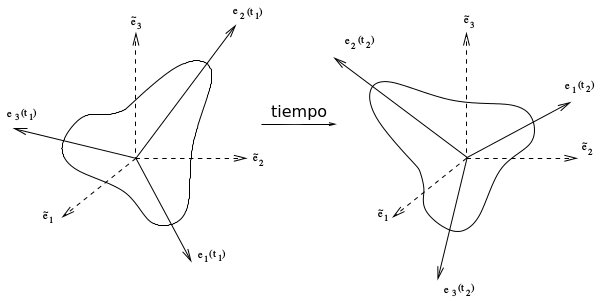
\includegraphics[scale=0.6]{problema5fig1}
 \caption{El marco de referencia estático y el marco de referencia en movimiento.}
\end{figure}

Debido a que ambos ejes son ortogonales, tenemos que 

\begin{equation}
 \tilde{\mathbf{e}}_a \cdot \tilde{\mathbf{e}}_b = \delta_{ab}, \quad \mathbf{e}_a(t) \cdot \mathbf{e}_b(t) = \delta_{ab}.
\end{equation}

\proposicion Para todo $t$, existe una matriz ortogonal única $R(t)$ con componentes 
$R_{ab}(t)$ tal que $\mathbf{e}_a(t) = R_{ab}(t)\tilde{\mathbf{e}}_b$.

\vspace{.3cm}

\prueba $\mathbf{e}_a \cdot \mathbf{e}_b = \delta_{ab} \Rightarrow R_{ac}R_{bd} 
(\tilde{\mathbf{e}}_c\cdot\tilde{\mathbf{e}}_d) = \delta_{ab} \Rightarrow R_{ac}R_{bc} = 
\delta_{ab}$ o, en otras palabras, $(R^TR)_{ab} = \delta_{ab}$ lo cual establece que 
$R$ es ortogonal. La unicidad de $R$ proviene de la construcción $R_{ab} = \mathbf{e}_a \cdot 
\tilde{\mathbf{e}}_b$.

$\hspace{12cm} \square$

\vspace{.3cm}

Entonces mientras el cuerpo rígido rota, esta rotación es descrita por una matriz 
$3\times 3$ ortogonal y dependiente del tiempo $R(t)$. Debido a la propiedad de 
las matrices $R$, $R_{ac}R_{bc} = \delta_{ab}$, y al hecho de que esta matriz es 
real, puede probarse sin dificultad que éstas tienen determinantes $\pm 1$. Debido 
a que todas las rotaciones físicas pueden ser alcanzadas continuamente de la 
la transformación idéntica (ángulo cero de rotación), y debido a que el determinante 
de esta es $+1$, entonces todas las matrices de rotación deben tener determinante $+1$, 
a este tipo de matrices se les llama matrices especiales. Entonces, cada familia uniparamétrica $R(t)$ describe un posible movimiento para 
el cuerpo, y llegamos a la siguiente conclusión:

\begin{center}
 $M$ = Variedad de configuración para  las rotaciones del cuerpo rígido = Espacio de las matrices 
 ortogonales especiales $\equiv$ \textbf{SO(3)}.
\end{center}

\vspace{.3cm}

Una matriz $3\times 3$ tiene $9$ componentes pero la condición de ortogonalidad $R^TR=1$
impone $6$ relaciones, por lo tanto la variedad de configuración es tridimensional, y 
por lo tanto necesitamos $3$ coordenadas generalizadas para parametrizar y describir 
completamente a $M$. Como probaremos en el siguiente teorema, estas coordenadas son 
los conocidos ángulos de Euler.

\teorema Una rotación arbitraria puede ser expresada como el producto de $3$ rotaciones 
sucesivas sobre (en general) $3$ ejes diferentes.

\vspace{.3cm}

\prueba Sean $\{{\tilde{\mathbf{e}}_a\}}$ los ejes del sistema estático y 
$\{{\mathbf{e}_a\}}$ los ejes anclados al cuerpo en rotación. Queremos encontrar 
la rotación $R$ tal que $\mathbf{e}_a = R_{ab}{\tilde{\mathbf{e}}_b}$. Podemos 
lograr esto en tres pasos

\begin{equation}
 \{{\tilde{\mathbf{e}}_a\}} \xrightarrow{R_3(\phi)} 
 \{{\mathbf{e}'_a\}} \xrightarrow{R_1(\theta)} 
 \{{\mathbf{e}''_a\}} \xrightarrow{R_3(\psi)} \{{\mathbf{e}_a\}}
\end{equation}

\textbf{Paso 1}: Rotación por un ángulo $\phi$ sobre el eje $\tilde{\mathbf{e}}_3$. 
Entonces $\mathbf{e}'_a = R_3(\phi)_{ab}\tilde{\mathbf{e}}_b$ con 

\begin{equation}
 R_3(\phi) = \begin{pmatrix}
              \cos{\phi} & \sen{\phi} & 0 \\
	      -\sen{\phi} & \cos{\phi} & 0 \\
	      0 & 0 & 1
	     \end{pmatrix}.
\end{equation}

\begin{figure}[H]
  \center 
  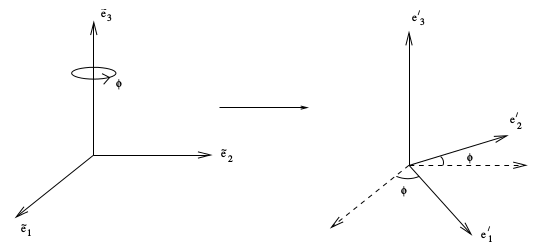
\includegraphics[scale=0.6]{problema5fig2}
  \caption{Paso 1: Rotación sobre $\tilde{\mathbf{e}}_e$ del marco de referencia 
  estático.}
\end{figure}

\textbf{Paso 2}: Rotación por un ángulo $\theta$ sobre el nuevo eje $\mathbf{e}'_1$. 
Este eje $\mathbf{e}'_1$ es conocido como la ``línea de nodos''. Escribimos entonces 
$\mathbf{e}''_a = R_1(\theta)\mathbf{e}'_b$ con 

\begin{equation}
 R_3(\theta) = \begin{pmatrix}
              1 & 0 & 0 \\
	      0 & \cos{\theta} & \sen{\theta} \\
	      0 & -\sen{\theta} & \cos{\theta}
	     \end{pmatrix}.
\end{equation}

\begin{figure}[H]
  \center 
  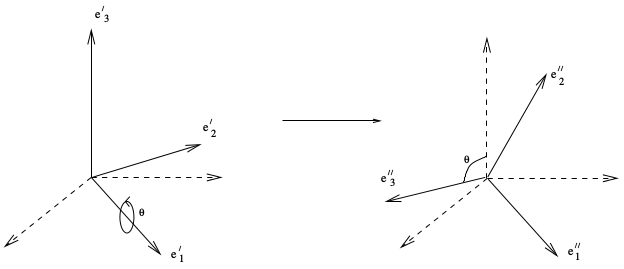
\includegraphics[scale=0.6]{problema5fig3}
  \caption{Paso 2: Rotación sobre el nuevo eje $\mathbf{e}'_1$.}
\end{figure}

\textbf{Paso 3}: Rotación por un ángulo $\psi$ sobre el nuevo eje $\mathbf{e}''_3$ 
entonces $\mathbf{e}_a = R_3(\psi)_{ab}\mathbf{e}''_b$ con 

\begin{equation}
 R_3(\psi) = \begin{pmatrix}
              \cos{\psi} & \sen{\psi} & 0 \\
	      -\sen{\psi} & \cos{\psi} & 0 \\
	      0 & 0 & 1
	     \end{pmatrix}.
\end{equation}

Poniendo todo esto junto tenemos que 

\begin{equation}
 R_{ab} (\phi,\theta,\psi) = [R_3(\phi)R_1(\theta)R_3(\psi)]_{ab}
\end{equation}

Los ángulos $\phi,\theta,\psi$ son los ángulos de Euler. Los cuales hemos demostrado 
entonces que forman un sistema de coordenadas para la variedad de configuración 
para las rotaciones de un cuerpo rígido, ya que podemos escribir la matriz $R(\phi,\theta,\psi)$
como 

\begin{equation*}
 R  = \begin{pmatrix}
              \cos{\psi}\cos{\phi} - \cos{\theta}\sen{\phi}\sen{\psi} & 
              \sen{\phi}\cos{\psi} + \cos{\theta}\sen{\psi}\cos{\phi} & 
              \sen{\theta}\sen{\psi} \\
	      -\cos{\psi}\sen{\psi} - \cos{\theta}\cos{\psi}\sen{\phi} & 
	      -\sen{\psi}\sen{\phi} + \cos{\theta}\cos{\psi}\cos{\phi} & 
	      \sen{\theta}\cos{\psi} \\
	      \sen{\theta}\sen{\phi} & -\sen{\theta}\cos{\phi} & \cos{\theta}
	     \end{pmatrix},
\end{equation*}

y esta cumple con las propiedades deseadas para probar el teorema que hemos propuesto 
y para formar un sistema de coordenadas locales para \textbf{SO(3)}. Cabe destacar 
que al utilizar estos ángulos para un problema concreto, debemos recordar que este 
sistema de coordenadas es similar a las coordenadas geográficas sobre la esfera: excluyen 
los polos y son multivaluadas en un meridiano.

$\hspace{12cm} \square$

\begin{thebibliography}{10}
\bibitem{lee}
J. Lee, \emph{Introduction to Smooth Manifolds}, Springer, 2006.
\bibitem{curtis}
W. Curtis y F. Miller, \emph{Differential Manifolds and Theoretical Physics}, Academic 
Press, 1985.
\bibitem{kosinski}
A. Kosinski, \emph{Differential Manifolds}, Academic Press, 1993.
\bibitem{torres}
G. Torres del Castillo, \emph{Differentiable Manifolds: A Theoretical Physics Approach}, 
Birkhäuser - Springer, 2012.
\end{thebibliography}


\end{document}
